% Practice Test 08 — Indiana Edition
% Questions: 30 (21 MC + 9 SA)
% Generated by scripts/generate_practice_tests.py

\begin{practiceQuestion}{1-3-q13}{mc}
\begin{questionText}
The table shows a proportional relationship. Find the missing value.

\begin{center}
\begin{tabular}{|c|c|}
\hline $x$ & $y$ \\ \hline $4$ & $14$ \\ $6$ & $?$ \\ $10$ & $35$ \\ \hline
\end{tabular}
\end{center}
\end{questionText}
\choiceA{$18$}
\choiceB{$20$}
\choiceC{$21$}
\choiceD{$24$}
\correctAnswer{C}
\explanation{$k = \frac{14}{4} = 3.5$. Missing value: $y = 3.5 \times 6 = 21$. Check: $\frac{35}{10} = 3.5$ \checkmark.}
\end{practiceQuestion}

\begin{practiceQuestion}{1-5-q21}{sa}
\begin{questionText}
A proportional line has slope $\frac{5}{3}$. Find $y$ when $x = 9$ and $x$ when $y = 25$.
\end{questionText}
\correctAnswer{$y = 15$ when $x = 9$; $x = 15$ when $y = 25$}
\explanation{$y = \frac{5}{3} \times 9 = 15$. For $y = 25$: $25 = \frac{5}{3}x$, so $x = 25 \times \frac{3}{5} = 15$.}
\end{practiceQuestion}

\begin{practiceQuestion}{1-6-q26}{gmc}
\begin{questionText}
The table shows the distance a bus travels over several hours. Using proportional reasoning, how far will the bus travel in $9$ hours?

\begin{center}
\begin{tabular}{|c|c|}
\hline
\textbf{Hours} & \textbf{Miles} \\ \hline
$2$ & $90$ \\ \hline
$5$ & $225$ \\ \hline
$7$ & $315$ \\ \hline
$9$ & $?$ \\ \hline
\end{tabular}
\end{center}
\end{questionText}
\choiceA{$360$ miles}
\choiceB{$385$ miles}
\choiceC{$405$ miles}
\choiceD{$450$ miles}
\correctAnswer{C}
\explanation{Rate: $90 \div 2 = 45$ mph. In $9$ hours: $45 \times 9 = 405$ miles.}
\end{practiceQuestion}

\begin{practiceQuestion}{2-2-q10}{mc}
\begin{questionText}
$96$ is $80\%$ of what number?
\end{questionText}
\choiceA{$76.8$}
\choiceB{$100$}
\choiceC{$116$}
\choiceD{$120$}
\correctAnswer{D}
\explanation{$\frac{96}{w} = \frac{80}{100}$. Cross-multiply: $80w = 9600$. Divide: $w = 120$.}
\end{practiceQuestion}

\begin{practiceQuestion}{2-5-q17}{mc}
\begin{questionText}
A freelance artist charges a $\$50$ base fee plus $7\%$ of the project value. For a $\$600$ project, what is the total charge?


\numberLine[100]{0}{700}
\end{questionText}
\choiceA{$\$42$}
\choiceB{$\$92$}
\choiceC{$\$107$}
\choiceD{$\$650$}
\correctAnswer{B}
\explanation{Percent fee: $600 \times 0.07 = \$42$. Total: $50 + 42 = \$92$.}
\end{practiceQuestion}

\begin{practiceQuestion}{2-7-q27}{gmc}
\begin{questionText}
The bar graph shows the estimated and actual heights of three trees. Which tree has the greatest percent error?

\begin{center}
\begin{tikzpicture}[scale=0.5]
  \draw[thick,->] (0,0) -- (0,7) node[above]{\small Height (ft)};
  \draw[thick,->] (0,0) -- (10.5,0);
  % Tree A: est 20, actual 25
  \fill[funBlue!60] (0.5,0) rectangle (1.5,4);
  \fill[funGreen!60] (1.5,0) rectangle (2.5,5);
  % Tree B: est 15, actual 12
  \fill[funBlue!60] (3.5,0) rectangle (4.5,3);
  \fill[funGreen!60] (4.5,0) rectangle (5.5,2.4);
  % Tree C: est 30, actual 28
  \fill[funBlue!60] (6.5,0) rectangle (7.5,6);
  \fill[funGreen!60] (7.5,0) rectangle (8.5,5.6);
  % Labels
  \node[below,font=\small] at (1.5,0) {Tree A};
  \node[below,font=\small] at (4.5,0) {Tree B};
  \node[below,font=\small] at (7.5,0) {Tree C};
  \foreach \y/\lab in {1/5,2/10,3/15,4/20,5/25,6/30} {
    \draw (-0.1,\y) -- (0.1,\y) node[left,font=\small,xshift=-2pt] {\lab};
  }
  % Values
  \node[above,font=\scriptsize,funBlue] at (1,4) {$20$};
  \node[above,font=\scriptsize,funGreen!80!black] at (2,5) {$25$};
  \node[above,font=\scriptsize,funBlue] at (4,3) {$15$};
  \node[above,font=\scriptsize,funGreen!80!black] at (5,2.4) {$12$};
  \node[above,font=\scriptsize,funBlue] at (7,6) {$30$};
  \node[above,font=\scriptsize,funGreen!80!black] at (8,5.6) {$28$};
  % Legend
  \fill[funBlue!60] (0.5,6.8) rectangle (1,7.2);
  \node[right,font=\scriptsize] at (1.1,7) {Estimated};
  \fill[funGreen!60] (3.5,6.8) rectangle (4,7.2);
  \node[right,font=\scriptsize] at (4.1,7) {Actual};
\end{tikzpicture}
\end{center}
\end{questionText}
\choiceA{Tree A ($20\%$)}
\choiceB{Tree B ($25\%$)}
\choiceC{Tree C ($7.1\%$)}
\choiceD{Trees A and B are tied}
\correctAnswer{B}
\explanation{A: $|20-25|/25 = 20\%$. B: $|15-12|/12 = 25\%$. C: $|30-28|/28 \approx 7.1\%$. Tree B has the greatest error.}
\end{practiceQuestion}

\begin{practiceQuestion}{3-1-q04}{mc}
\begin{questionText}
A number plus its opposite always equals which value?
\end{questionText}
\choiceA{$1$}
\choiceB{$-1$}
\choiceC{The number itself}
\choiceD{$0$}
\correctAnswer{D}
\explanation{A number and its opposite are additive inverses. For example, $5 + (-5) = 0$.}
\end{practiceQuestion}

\begin{practiceQuestion}{3-2-q12}{mc}
\begin{questionText}
What is $(-7) + 7 + (-3)$?
\end{questionText}
\choiceA{$-3$}
\choiceB{$3$}
\choiceC{$-17$}
\choiceD{$17$}
\correctAnswer{A}
\explanation{$(-7) + 7 = 0$ (opposites cancel). Then $0 + (-3) = -3$.}
\end{practiceQuestion}

\begin{practiceQuestion}{4-2-q25}{sa}
\begin{questionText}
Write an expression with three terms that simplifies to $4n + 7$.
\end{questionText}
\correctAnswer{Answers vary, e.g., $n + 3n + 7$ or $5n - n + 7$}
\explanation{Any expression whose like terms combine to give $4n + 7$ is correct. For example: $n + 3n + 7 = 4n + 7$.}
\end{practiceQuestion}

\begin{practiceQuestion}{4-3-q03}{mc}
\begin{questionText}
Expand $-2(3x + 7)$.
\end{questionText}
\choiceA{$-6x + 7$}
\choiceB{$-6x - 14$}
\choiceC{$-6x + 14$}
\choiceD{$6x - 14$}
\correctAnswer{B}
\explanation{$-2 \times 3x = -6x$ and $-2 \times 7 = -14$. Result: $-6x - 14$.}
\end{practiceQuestion}

\begin{practiceQuestion}{5-4-q30}{gsa}
\begin{questionText}
A number line shows a point at $x$. The equation $\dfrac{x}{4} + 1.5 = 5$ tells you how to find $x$. Solve and identify where $x$ is on the number line.

\begin{center}
\begin{tikzpicture}[scale=0.45]
  \draw[thick,->] (-2,0) -- (18,0);
  \foreach \x in {0,2,...,16} {
    \draw (\x,0.2) -- (\x,-0.2) node[below] {$\x$};
  }
  \node[above,funBlue] at (14,0.5) {$x = \;?$};
  \draw[thick,->,funBlue] (14,0.4) -- (14,0.1);
\end{tikzpicture}
\end{center}
\end{questionText}
\correctAnswer{$x = 14$}
\explanation{Subtract $1.5$: $\frac{x}{4} = 3.5$. Multiply by $4$: $x = 14$. The point is at $14$ on the number line.}
\end{practiceQuestion}

\begin{practiceQuestion}{5-5-q19}{sa}
\begin{questionText}
Solve $6x + 9 > 45$.
\end{questionText}
\correctAnswer{$x > 6$}
\explanation{Subtract $9$: $6x > 36$. Divide by $6$: $x > 6$.}
\end{practiceQuestion}

\begin{practiceQuestion}{5-6-q21}{sa}
\begin{questionText}
Solve $\dfrac{n}{3} + 2 \leq 6$. Describe the graph.
\end{questionText}
\correctAnswer{$n \leq 12$; closed circle at $12$, shade left}
\explanation{Subtract $2$: $\frac{n}{3} \leq 4$. Multiply by $3$: $n \leq 12$. Closed circle at $12$, shade left.}
\end{practiceQuestion}

\begin{practiceQuestion}{6-1-q07}{mc}
\begin{questionText}
A park is $120$ m long. On a scale drawing, it is $8$ cm long. What scale does the drawing use?
\end{questionText}
\choiceA{$1$ cm $= 10$ m}
\choiceB{$1$ cm $= 12$ m}
\choiceC{$1$ cm $= 15$ m}
\choiceD{$1$ cm $= 20$ m}
\correctAnswer{C}
\explanation{$120 \div 8 = 15$. The scale is $1$ cm $= 15$ m.}
\end{practiceQuestion}

\begin{practiceQuestion}{6-3-q02}{mc}
\begin{questionText}
Can you draw a triangle with sides $5$ cm, $5$ cm, and $5$ cm?
\end{questionText}
\choiceA{No, it is impossible}
\choiceB{Yes, exactly one triangle}
\choiceC{Yes, more than one triangle}
\choiceD{Yes, but only if one angle is $90°$}
\correctAnswer{B}
\explanation{All three inequality checks pass ($5 + 5 = 10 > 5$). Three equal sides (SSS) produce exactly one equilateral triangle.}
\end{practiceQuestion}

\begin{practiceQuestion}{6-4-q24}{sa}
\begin{questionText}
You are given two sides ($5$ cm and $7$ cm) and the included angle ($90°$). Is the resulting triangle unique? What type of triangle is it?
\end{questionText}
\correctAnswer{Yes, unique; it is a right triangle}
\explanation{SAS produces a unique triangle. The included angle of $90°$ makes it a right triangle with legs $5$ cm and $7$ cm.}
\end{practiceQuestion}

\begin{practiceQuestion}{6-5-q28}{gmc}
\begin{questionText}
The diagram shows a triangular prism. A cut is made parallel to the triangular base (shown as the shaded region). What is the cross-section?

\begin{center}
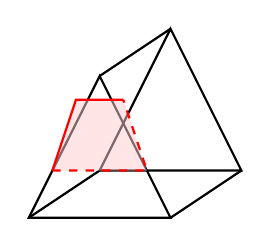
\begin{tikzpicture}[scale=0.6]
  % Front triangle
  \draw[thick] (0,0) -- (3,0) -- (1.5,3) -- cycle;
  % Back triangle
  \draw[thick] (1.5,1) -- (4.5,1) -- (3,4) -- cycle;
  % Connecting edges
  \draw[thick] (0,0) -- (1.5,1);
  \draw[thick] (3,0) -- (4.5,1);
  \draw[thick] (1.5,3) -- (3,4);
  % Cross section
  \fill[red!20,opacity=0.5] (0.5,1) -- (2.5,1) -- (2,2.5) -- (1,2.5) -- cycle;
  \draw[thick,red,dashed] (0.5,1) -- (2.5,1) -- (2,2.5);
  \draw[thick,red] (0.5,1) -- (1,2.5) -- (2,2.5);
\end{tikzpicture}
\end{center}
\end{questionText}
\choiceA{Rectangle}
\choiceB{Triangle}
\choiceC{Circle}
\choiceD{Hexagon}
\correctAnswer{B}
\explanation{A cut parallel to the base of a prism gives a shape congruent to the base. Since the base is a triangle, the cross-section is a triangle.}
\end{practiceQuestion}

\begin{practiceQuestion}{6-6-q15}{mc}
\begin{questionText}
Which pair of angles is complementary?
\end{questionText}
\choiceA{$50°$ and $130°$}
\choiceB{$55°$ and $35°$}
\choiceC{$60°$ and $60°$}
\choiceD{$45°$ and $135°$}
\correctAnswer{B}
\explanation{Complementary angles sum to $90°$. Only $55 + 35 = 90$.}
\end{practiceQuestion}

\begin{practiceQuestion}{6-7-q04}{mc}
\begin{questionText}
Point $D(2, 6)$ is rotated $90°$ clockwise about the origin. What are the coordinates of $D'$?
\end{questionText}
\choiceA{$(-6, 2)$}
\choiceB{$(6, -2)$}
\choiceC{$(-2, -6)$}
\choiceD{$(6, 2)$}
\correctAnswer{B}
\explanation{$90°$ clockwise: $(x, y) \to (y, -x)$. $(2, 6) \to (6, -2)$.}
\end{practiceQuestion}

\begin{practiceQuestion}{7-3-q17}{mc}
\begin{questionText}
What is the area of a circle with a radius of $1.5$ meters? Use $\pi \approx 3.14$.
\end{questionText}
\choiceA{$4.71$ m$^2$}
\choiceB{$7.065$ m$^2$}
\choiceC{$9.42$ m$^2$}
\choiceD{$14.13$ m$^2$}
\correctAnswer{B}
\explanation{$A = \pi r^2 = 3.14 \times (1.5)^2 = 3.14 \times 2.25 = 7.065$ m$^2$.}
\end{practiceQuestion}

\begin{practiceQuestion}{7-4-q26}{gmc}
\begin{questionText}
What is the area of the shaded composite figure on the grid? Each square is $1$ cm by $1$ cm.

\begin{center}
\begin{tikzpicture}[scale=0.5]
  \draw[step=1,gray!30,thin] (0,0) grid (10,7);
  \fill[funBlue!20] (1,1) -- (9,1) -- (9,4) -- (6,4) -- (6,6) -- (4,6) -- (4,4) -- (1,4) -- cycle;
  \draw[thick,funBlue] (1,1) -- (9,1) -- (9,4) -- (6,4) -- (6,6) -- (4,6) -- (4,4) -- (1,4) -- cycle;
  \node[below] at (1,1) {\small $(1{,}1)$};
  \node[below] at (9,1) {\small $(9{,}1)$};
  \node[right] at (9,4) {\small $(9{,}4)$};
  \node[right] at (6,4) {\small $(6{,}4)$};
  \node[above] at (6,6) {\small $(6{,}6)$};
  \node[above] at (4,6) {\small $(4{,}6)$};
  \node[left] at (4,4) {\small $(4{,}4)$};
  \node[left] at (1,4) {\small $(1{,}4)$};
\end{tikzpicture}
\end{center}
\end{questionText}
\choiceA{$24$ cm$^2$}
\choiceB{$28$ cm$^2$}
\choiceC{$32$ cm$^2$}
\choiceD{$36$ cm$^2$}
\correctAnswer{B}
\explanation{Bottom rectangle: $8 \times 3 = 24$ cm$^2$. Top rectangle: $2 \times 2 = 4$ cm$^2$. Total: $24 + 4 = 28$ cm$^2$.}
\end{practiceQuestion}

\begin{practiceQuestion}{7-5-q20}{sa}
\begin{questionText}
A cube has a side length of $7$ m. What is its surface area?
\end{questionText}
\correctAnswer{$294$ m$^2$}
\explanation{$SA = 6s^2 = 6 \times 49 = 294$ m$^2$.}
\end{practiceQuestion}

\begin{practiceQuestion}{7-6-q16}{mc}
\begin{questionText}
A rectangular prism has a volume of $240$ cm$^3$. Its base is $8$ cm by $6$ cm. What is the height?
\end{questionText}
\choiceA{$4$ cm}
\choiceB{$5$ cm}
\choiceC{$6$ cm}
\choiceD{$10$ cm}
\correctAnswer{B}
\explanation{$B = 8 \times 6 = 48$ cm$^2$. $h = V \div B = 240 \div 48 = 5$ cm.}
\end{practiceQuestion}

\begin{practiceQuestion}{8-1-q30}{gsa}
\begin{questionText}
The table shows the results of a random sample of $80$ people about their preferred pet.

\begin{center}
\begin{tabular}{|l|c|}
\hline
\textbf{Pet} & \textbf{Number} \\
\hline
Dog & $32$ \\
\hline
Cat & $24$ \\
\hline
Fish & $12$ \\
\hline
Bird & $8$ \\
\hline
Other & $4$ \\
\hline
\end{tabular}
\end{center}

What percent of the sample prefers cats? If the population is $5{,}000$, predict how many prefer cats.
\end{questionText}
\correctAnswer{$30\%$; $1{,}500$ people}
\explanation{$\frac{24}{80} = 0.30 = 30\%$. Then $30\%$ of $5{,}000 = 1{,}500$.}
\end{practiceQuestion}

\begin{practiceQuestion}{8-3-q01}{mc}
\begin{questionText}
Class A has a mean test score of $78$ and Class B has a mean test score of $85$. What can you conclude?
\end{questionText}
\choiceA{Every student in Class B scored higher than every student in Class A}
\choiceB{Class B scored higher on average than Class A}
\choiceC{Class A and Class B have the same scores}
\choiceD{Class A has more students than Class B}
\correctAnswer{B}
\explanation{The mean tells us the average performance. Class B scored higher on average, but individual scores may overlap.}
\end{practiceQuestion}

\begin{practiceQuestion}{8-4-q14}{mc}
\begin{questionText}
Data: $42, 45, 47, 50, 53, 55, 58$. Find $Q_1$ and $Q_3$.
\end{questionText}
\choiceA{$Q_1 = 45$, $Q_3 = 55$}
\choiceB{$Q_1 = 42$, $Q_3 = 58$}
\choiceC{$Q_1 = 47$, $Q_3 = 53$}
\choiceD{$Q_1 = 44$, $Q_3 = 56$}
\correctAnswer{A}
\explanation{Median $= 50$. Lower half: $42, 45, 47$, so $Q_1 = 45$. Upper half: $53, 55, 58$, so $Q_3 = 55$.}
\end{practiceQuestion}

\begin{practiceQuestion}{8-7-q03}{mc}
\begin{questionText}
A double bar graph is used to:
\end{questionText}
\choiceA{Show one data set over time}
\choiceB{Compare two data sets using side-by-side bars}
\choiceC{Show parts of a whole}
\choiceD{Display individual data points}
\correctAnswer{B}
\explanation{Double bar graphs place two sets of bars side by side for each category so you can compare them directly.}
\end{practiceQuestion}

\begin{practiceQuestion}{9-4-q21}{sa}
\begin{questionText}
A bag has $6$ red, $4$ blue, and $10$ white marbles. Write the probability model by listing $P(\text{red})$, $P(\text{blue})$, and $P(\text{white})$ as fractions in simplest form.
\end{questionText}
\correctAnswer{$P(\text{red}) = \frac{3}{10}$, $P(\text{blue}) = \frac{1}{5}$, $P(\text{white}) = \frac{1}{2}$}
\explanation{Total: $20$. $P(\text{red}) = \frac{6}{20} = \frac{3}{10}$, $P(\text{blue}) = \frac{4}{20} = \frac{1}{5}$, $P(\text{white}) = \frac{10}{20} = \frac{1}{2}$.}
\end{practiceQuestion}

\begin{practiceQuestion}{9-6-q26}{gmc}
\begin{questionText}
The table shows all possible sums when two dice are rolled. What is the probability of rolling a sum of $8$?

\begin{center}
\begin{tabular}{|c|c|c|c|c|c|c|}
\hline
$+$ & \textbf{1} & \textbf{2} & \textbf{3} & \textbf{4} & \textbf{5} & \textbf{6} \\
\hline
\textbf{1} & $2$ & $3$ & $4$ & $5$ & $6$ & $7$ \\
\hline
\textbf{2} & $3$ & $4$ & $5$ & $6$ & $7$ & \cellcolor{funBlue!20}$8$ \\
\hline
\textbf{3} & $4$ & $5$ & $6$ & $7$ & \cellcolor{funBlue!20}$8$ & $9$ \\
\hline
\textbf{4} & $5$ & $6$ & $7$ & \cellcolor{funBlue!20}$8$ & $9$ & $10$ \\
\hline
\textbf{5} & $6$ & $7$ & \cellcolor{funBlue!20}$8$ & $9$ & $10$ & $11$ \\
\hline
\textbf{6} & $7$ & \cellcolor{funBlue!20}$8$ & $9$ & $10$ & $11$ & $12$ \\
\hline
\end{tabular}
\end{center}
\end{questionText}
\choiceA{$\frac{4}{36}$}
\choiceB{$\frac{5}{36}$}
\choiceC{$\frac{6}{36}$}
\choiceD{$\frac{8}{36}$}
\correctAnswer{B}
\explanation{Outcomes with sum $8$: $(2,6), (3,5), (4,4), (5,3), (6,2)$ — that is $5$. $P = \frac{5}{36}$.}
\end{practiceQuestion}

\begin{practiceQuestion}{9-7-q18}{mc}
\begin{questionText}
In a simulation of $100$ free throws, a basketball player makes $78$. If the player's actual success rate is $75\%$, is the simulation result reasonable?
\end{questionText}
\choiceA{No, any difference means the simulation is wrong}
\choiceB{Yes, $78\%$ is close to $75\%$, which is expected variation}
\choiceC{No, because $78$ is not equal to $75$}
\choiceD{Yes, but only if exactly $75$ are made}
\correctAnswer{B}
\explanation{$\frac{78}{100} = 0.78$ vs. theoretical $0.75$. A small difference in $100$ trials is normal and expected.}
\end{practiceQuestion}
